\subsection{Треугольная функция}

Рассмотрим семейство функций
\begin{equation}
    f(t) = \begin{cases}
        a - |at / b|, & |t| \le b, \\
        0, & |t| > b
    \end{cases}
    \label{eq:triangle_function}
\end{equation}

\subsubsection{Графики исходных функций}

\begin{figure}[ht!]
    \centering
    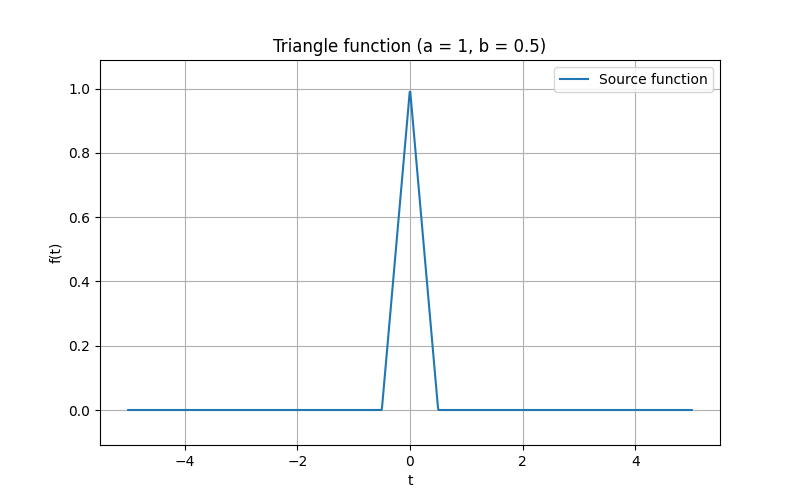
\includegraphics[width=\textwidth]{media/triangle_1.png}
    \caption{График прямоугольной функции $f(t)$ при $a = 1$, $b = 0.5$}
    \label{fig:triangle_1}
\end{figure}

\begin{figure}[ht!]
    \centering
    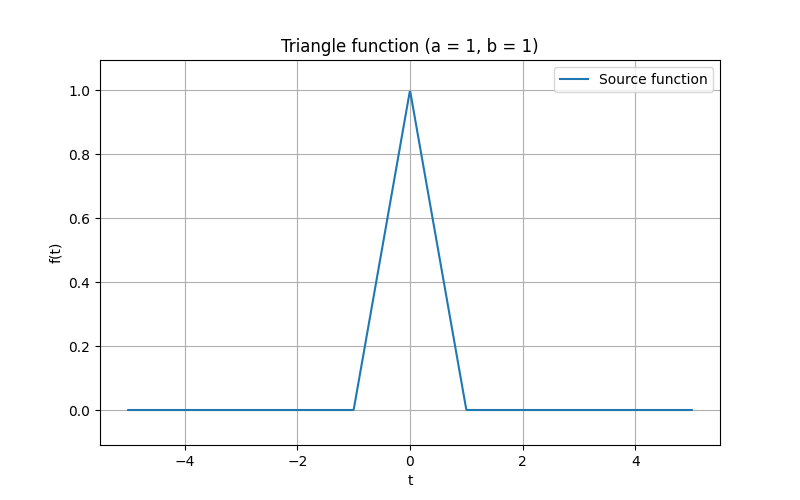
\includegraphics[width=\textwidth]{media/triangle_2.png}
    \caption{График прямоугольной функции $f(t)$ при $a = 1$, $b = 1$}
    \label{fig:triangle_2}
\end{figure}

\begin{figure}[ht!]
    \centering
    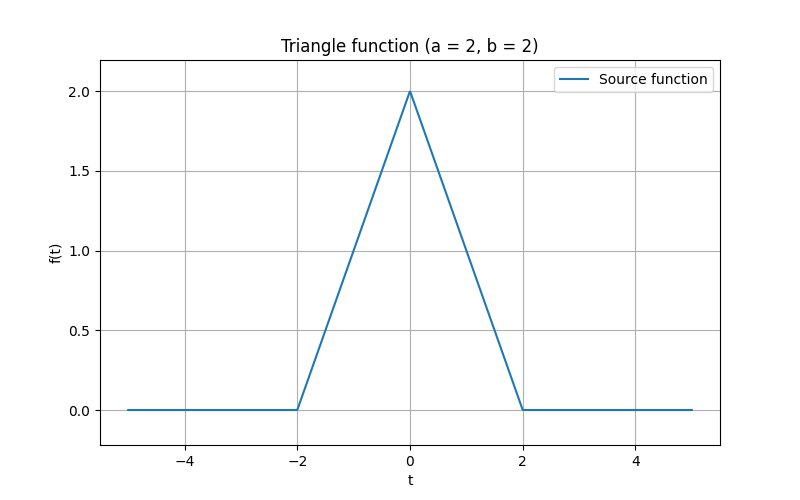
\includegraphics[width=\textwidth]{media/triangle_3.png}
    \caption{График прямоугольной функции $f(t)$ при $a = 2$, $b = 2$}
    \label{fig:triangle_3}
\end{figure}

\subsubsection{Нахождение образа функции}
Согласно формуле \eqref{eq:image_from_function}, Фурье образ функции $f(t)$ задается следующим выражением:
\begin{multline}
    \hat{f}(\omega) = \frac{1}{\sqrt{2\pi}} \int_{-\infty}^{\infty} f(t) e^{-i\omega t} dt = \frac{1}{\sqrt{2\pi}} \int_{-b}^{b} (a - |at / b|) e^{-i\omega t} dt = \\
    \frac{1}{\sqrt{2\pi}} \left(\int_{-b}^{0}{(a + \frac{at}{b}) e^{-i\omega t}} dt + \int_{0}^{b}{(a - \frac{at}{b}) e^{-i\omega t}} dt\right) =
    \frac{1}{\sqrt{2 \pi}} \left(\frac{a(ib\omega - e^{ib\omega} + 1)}{b \omega^2} + \frac{a(-ib\omega - e^{-ib\omega} + 1)}{b\omega^2} \right) = \\
    \frac{1}{\sqrt{2\pi}} \left( \frac{a (-e^{ib\omega} - e^{-ib\omega} + 2)} {b\omega^2} \right) = \frac{1}{\sqrt{2\pi}} \frac{4a \sin(\frac{b\omega}{2})^2}{b \omega^2}  = \frac{4a\sin(\frac{b\omega}{2})^2}{\sqrt{2\pi} b \omega^2} = \frac{ab}{\sqrt{2\pi}} \sinc^2\left(\frac{b\omega}{2}\right)
    \label{eq:truangle_image}
\end{multline}

для $a = 1$, $b = 0.5$:
\begin{equation}
    \hat{f_1}(\omega) = \frac{1}{\sqrt{2\pi}} \sinc^2\left(\frac{\omega}{4}\right)
\end{equation}

для $a = 1$, $b = 1$:
\begin{equation}
    \hat{f_2}(\omega) = \frac{1}{\sqrt{2\pi}} \sinc^2\left(\frac{\omega}{2}\right)
\end{equation}

для $a = 2$, $b = 2$:
\begin{equation}
    \hat{f_3}(\omega) = \frac{4}{\sqrt{2\pi}} \sinc^2\left(\omega\right)
\end{equation}

\subsubsection{Графики образов функций}
Графики образов треугольной функции при различных значениях $a$ и $b$ представлены на рисунках \ref{fig:triangle_1_image}, \ref{fig:triangle_2_image} и \ref{fig:triangle_3_image}.

\begin{figure}[ht!]
    \centering
    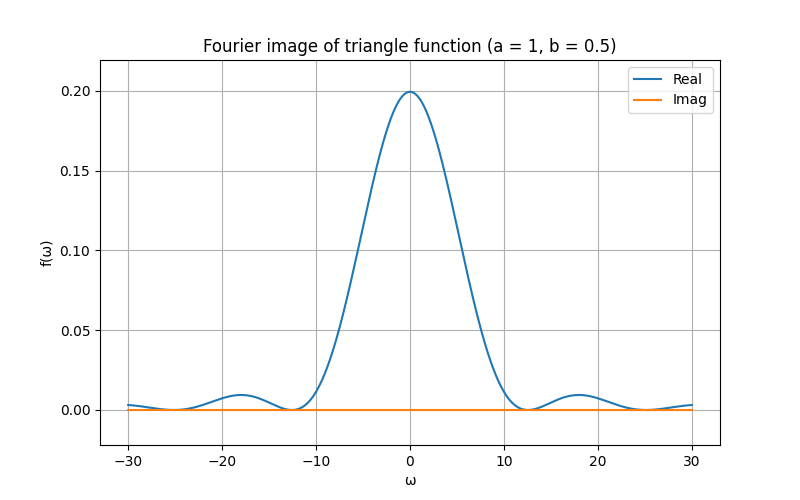
\includegraphics[width=\textwidth]{media/triangle_1_image.png}
    \caption{График Фурье образа треугольной функции $\hat{f}(\omega)$ при $a = 1$, $b = 0.5$}
    \label{fig:triangle_1_image}
\end{figure}

\begin{figure}[ht!]
    \centering
    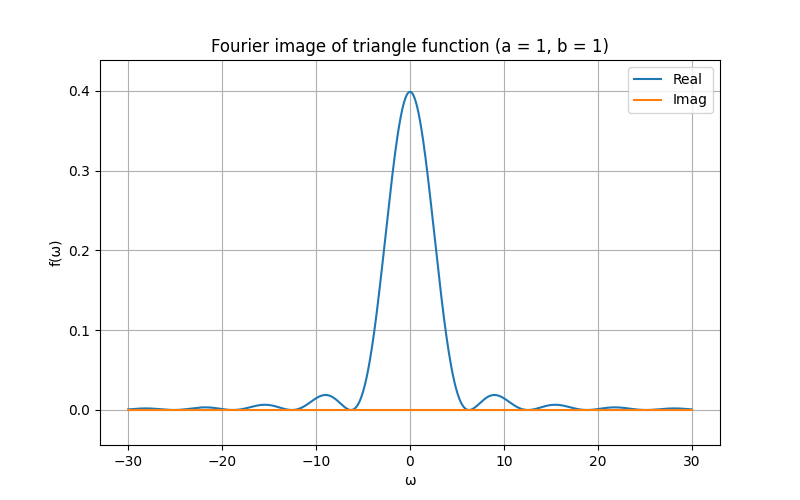
\includegraphics[width=\textwidth]{media/triangle_2_image.png}
    \caption{График Фурье образа треугольной функции $\hat{f}(\omega)$ при $a = 1$, $b = 1$}
    \label{fig:triangle_2_image}
\end{figure}

\begin{figure}[ht!]
    \centering
    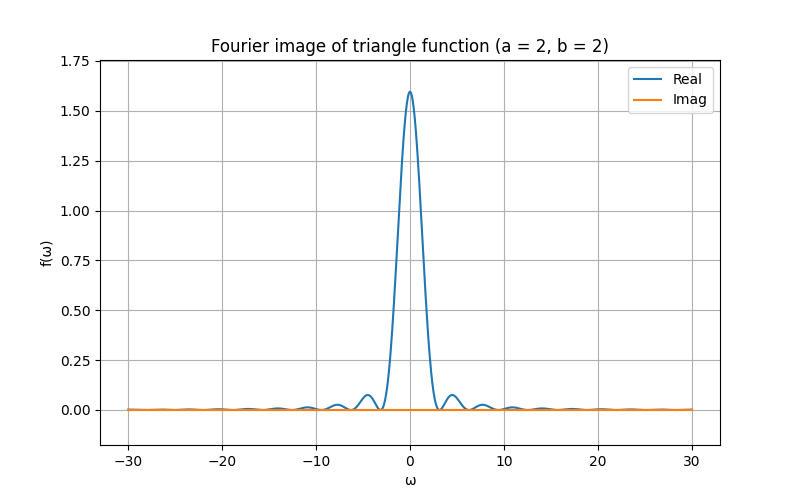
\includegraphics[width=\textwidth]{media/triangle_3_image.png}
    \caption{График Фурье образа треугольной функции $\hat{f}(\omega)$ при $a = 2$, $b = 2$}
    \label{fig:triangle_3_image}
\end{figure}

\FloatBarrier
\subsubsection{Проверка равенства Парсеваля}
Проверим равенство Парсеваля (см. формулу~\eqref{eq:parseval_indentity}). Для этого воспользуемся функцией \texttt{parseval\_check}.
\begin{table}[ht!]
    \centering
    \begin{tabular}{|c|c|}
        \hline
        $\displaystyle\int_{-100}^{100}{|f(t)|^2}$ & $\displaystyle\int_{-100}^{100}{|\hat{f_1}(\omega)|^2}$ \\
        \hline
        0.3333 & 0.3333 \\
        \hline
    \end{tabular}
    \caption{Результаты проверки равенства Парсеваля для треугольной функции $f(t)$ при $a = 1$, $b = 0.5$}
    \label{tab:triangle_1_parseval_check}
\end{table}

\begin{table}[ht!]
    \centering
    \begin{tabular}{|c|c|}
        \hline
        $\displaystyle\int_{-100}^{100}{|f(t)|^2}$ & $\displaystyle\int_{-100}^{100}{|\hat{f_2}(\omega)|^2}$ \\
        \hline
        0.6666 & 0.6666 \\
        \hline
    \end{tabular}
    \caption{Результаты проверки равенства Парсеваля для треугольной функции $f(t)$ при $a = 1$, $b = 1$}
    \label{tab:triangle_2_parseval_check}
\end{table}

\begin{table}[ht!]
    \centering
    \begin{tabular}{|c|c|}
        \hline
        $\displaystyle\int_{-100}^{100}{|f(t)|^2}$ & $\displaystyle\int_{-100}^{100}{|\hat{f_3}(\omega)|^2}$ \\
        \hline
        5.3333 & 5.3333 \\
        \hline
    \end{tabular}
    \caption{Результаты проверки равенства Парсеваля для треугольной функции $f(t)$ при $a = 2$, $b = 2$}
    \label{tab:triangle_3_parseval_check}
\end{table}

Видим, что во всех случаях равенство Парсеваля выполняется с высокой точностью.

\subsubsection{Анализ результатов}
Влияние параметров $a$ и $b$ на исходную функцию и ее Фурье образ определяются из формулы \eqref{eq:triangle_function} и выражения для Фурье образа \eqref{eq:truangle_image}. Параметр $a$ определяет высоту треугольной функции, а параметр $b$ --- ширину основания. В образе функции видно, что при увеличении параметра $a$ амплитуда образа увеличивается, а при увеличении параметров $a$ и $b$ амплитуда увеличивается, при увеличении параметра $b$ увеличивается частота. 

Принцип неопределенности, как и с прошлом случае, можно наблюдать как уменьшение ширины образа при увеличении основания треугольника.